\documentclass[20pt, a0paper, landscape]{tikzposter}

% ---------- Packages ----------
\usepackage[T1]{fontenc}
\usepackage[utf8]{inputenc}
\usepackage{lmodern}
\usepackage{microtype}
\usepackage{amsmath,amssymb}
\usepackage{graphicx}
\usepackage{booktabs,array,colortbl}
\usepackage{enumitem}
\usepackage{tikz}
\usetikzlibrary{calc,positioning,shapes,arrows.meta}

% ---------- ALU palette ----------
\definecolor{ALUBlue}{HTML}{002E6D}
\definecolor{ALUBlueLight}{HTML}{EAF1FB}
\definecolor{ALUBlueLine}{HTML}{BFD0EA}
\definecolor{ALUText}{HTML}{1E2A38}
\definecolor{ALUMuted}{HTML}{5C6B7A}
\definecolor{ALUWhite}{HTML}{FFFFFF}
\definecolor{ALUAccent}{HTML}{D9E6F7}
\definecolor{FBGreen}{HTML}{166534}
\definecolor{FBAmber}{HTML}{92400E}
\definecolor{FBAmberLight}{HTML}{FEF3C7}
\definecolor{FBOrange}{HTML}{C2410C}

% ---------- Theme ----------
\usetheme{Simple}
\usecolorstyle{Default}
\usebackgroundstyle{Default}
\colorlet{backgroundcolor}{ALUWhite}
\colorlet{framecolor}{ALUBlueLine}
\colorlet{titlefgcolor}{white}
\colorlet{titlebgcolor}{ALUBlue}
\colorlet{blocktitlebgcolor}{ALUBlue}
\colorlet{blocktitlefgcolor}{white}
\colorlet{blockbodybgcolor}{white}
\colorlet{blockbodyfgcolor}{ALUText}

% ---------- Tight spacing ----------
\setlength{\parindent}{0pt}
\setlength{\parskip}{0pt}
\linespread{0.93}
\setlist[itemize]{leftmargin=1em,itemsep=0pt,topsep=0pt,parsep=0pt,partopsep=0pt}
\setlist[enumerate]{leftmargin=1.3em,itemsep=0pt,topsep=0pt,parsep=0pt,partopsep=0pt}

% ---------- Compact block style ----------
\defineblockstyle{ALUBlock}{
    titlewidthscale=1, bodywidthscale=1, roundedcorners=12,
    titleleft, titleoffsetx=0mm, titleoffsety=0mm,
    bodyoffsetx=0mm, bodyoffsety=2mm,
    bodyverticalshift=2mm, linewidth=0.8mm
}{
    \draw[rounded corners=12pt, line width=0.9mm, color=ALUBlueLine, fill=white]
      (blockbody.south west) rectangle (blockbody.north east);
    \ifBlockHasTitle
      \draw[rounded corners=12pt, line width=0mm, fill=ALUBlue]
      (blocktitle.south west) rectangle (blocktitle.north east);
    \fi
}
\useblockstyle{ALUBlock}

% ---------- Helpers ----------
\newcommand{\takeawaybox}[1]{%
  \begin{center}
  \fcolorbox{ALUBlueLine}{ALUBlueLight}{%
    \parbox{0.93\linewidth}{\centering\bfseries #1}%
  }\end{center}\vspace{0.1em}%
}

\newcommand{\metricbox}[3]{%
  \fcolorbox{#3}{#3!12}{%
    \parbox[c][2.4cm][c]{0.295\linewidth}{%
      \centering\bfseries\LARGE\color{#3} #1\\[0.1em]%
      \small\color{ALUText} #2%
    }%
  }%
}

\newcommand{\screenshotbox}[2][3.0cm]{%
  \begin{center}
  \IfFileExists{#2.png}{%
    \includegraphics[width=0.97\linewidth,height=#1,keepaspectratio]{#2.png}%
  }{%
    \fcolorbox{ALUBlueLine}{ALUBlueLight}{%
      \parbox[c][#1][c]{0.95\linewidth}{\centering\small\bfseries\color{ALUBlue}[Screenshot: #2]}%
    }%
  }\end{center}%
}

% ---------- Title (compact) ----------
\title{\Large\textbf{FarmBridge} --- Direct Farmer-to-Buyer Agricultural Marketplace for Rwanda}
\author{\normalsize
  Mugisha Moses (PM) \quad
  Nkingi Gakindi Chris (Lead Dev) \quad
  Hakizimana Chris Marcel (DB) \quad
  Ineza Ghislaine (UI/UX) \quad
  Kamy Uwambaye (Research)%
}
\institute{\small
  African Leadership University \textbar\
  BSc (Hons) Software Engineering \textbar\
  Foundations Project \textbar\ February -- March 2026%
}
\titlegraphic{
\includegraphics[height=2.8cm]{alu-logo-white-full.png}}

\begin{document}
\maketitle
\vspace{-0.3cm}

\begin{columns}

%% ===== LEFT (0.30) =====
\column{0.30}

\block{1. Problem, Context \& Users}{
\takeawaybox{Rwanda's 5.4M smallholder farmers lose 30--60\% of crop value to middlemen --- not because they produce less, but because they can't reach fair markets.}

Agriculture drives \textbf{24\% of Rwanda's GDP} and employs 70\% of its workforce. Farmers (avg.\ 1~ha) are locked out of fair markets because:
\begin{itemize}
  \item Intermediaries capture 30--60\% of crop value
  \item Post-harvest losses reach 40\% sub-Saharan Africa (FAO, 2022)
  \item Existing platforms (eHaho, Farmzone) are English-only, require internet, and have no in-app negotiation
\end{itemize}
\vspace{0.1em}
\begin{tabular}{>{\small\bfseries\color{ALUBlue}}p{0.18\linewidth}p{0.75\linewidth}}
Users & Smallholder farmers (Musanze, Nyagatare, Huye), verified buyers, admins \\[0.1em]
Gap   & No Rwanda platform offers offline + Kinyarwanda + direct negotiation \\
\end{tabular}
}

\block{2. Objectives \& Scope}{
\begin{itemize}
  \item \textbf{Aim:} Bilingual (EN/Kinyarwanda) PWA connecting farmers directly with verified buyers at zero fee.
  \item \textbf{Obj.\ 1:} Offline-first 3-tier architecture (Service Workers + IndexedDB).
  \item \textbf{Obj.\ 2:} Six modules --- auth, listings, marketplace, real-time negotiation, orders, admin.
  \item \textbf{Obj.\ 3:} $<$3\,s load, 90\% task completion, $\geq$4/5 usability score.
\end{itemize}
\vspace{0.1em}
{\small\begin{tabular}{>{\bfseries\color{FBGreen}}p{0.16\linewidth}p{0.77\linewidth}}
In     & PWA, listings, search, chat + price proposals, order lifecycle, Stripe + MoMo, ratings, notifications \\[0.1em]
\rowcolor{FBAmberLight}
Out    & GPS tracking, hardware, mobile-money wallet management \\
\end{tabular}}
}

\block{3. Project Metadata \& Team}{
{\small\begin{tabular}{>{\bfseries}p{0.24\linewidth}p{0.70\linewidth}}
Team      & Moses (PM) $\cdot$ Chris N.\ (Dev) $\cdot$ Chris H.\ (DB) $\cdot$ Ghislaine (UX) $\cdot$ Kamy (Research) \\[0.1em]
Programme & BSc Software Engineering, ALU Rwanda, Cohort 2026 \\[0.1em]
Duration  & 12-week sprint (Feb -- Mar 2026) \\[0.1em]
Frontend  & Next.js 16, React 19, Tailwind CSS, shadcn/ui \\[0.1em]
Backend   & NestJS 11, Prisma ORM, Socket.io, BullMQ \\[0.1em]
Data      & PostgreSQL (8 entities), Redis (cache + WS adapter) \\[0.1em]
External  & Cloudinary, Firebase FCM, Stripe, Flutterwave \\
\end{tabular}}
}

\block{4. Constraints \& Design Decisions}{
{\small\begin{tabular}{>{\bfseries\color{ALUBlue}}p{0.28\linewidth}p{0.65\linewidth}}
\rowcolor{ALUBlueLight}
Constraint & Design Response \\[0.06em]
\midrule
Rural connectivity   & Offline-first PWA: Service Workers + IndexedDB background sync \\[0.1em]
Low digital literacy & Icon UI, EN$\leftrightarrow$Kinyarwanda toggle, onboarding walkthrough \\[0.1em]
No bank card         & Flutterwave: M-Pesa, MTN Mobile Money, Orange Money \\[0.1em]
Data security        & JWT access+refresh, bcrypt, Helmet, input sanitisation \\[0.1em]
Real-time chat       & Socket.io + Redis adapter (horizontally scalable) \\[0.1em]
Image bandwidth      & Cloudinary CDN: auto-resize, compression, lazy loading \\
\end{tabular}}
\vspace{0.1em}
{\small\textbf{Trade-off:} Offline reliability prioritised over feature richness --- core actions queue locally and sync on reconnect.}
}


%% ===== MIDDLE (0.40) =====
\column{0.40}

\block{5. Proposed Solution \& System Architecture}{
\takeawaybox{FarmBridge removes the middleman: farmers list $\rightarrow$ buyers negotiate directly $\rightarrow$ orders placed, paid, and tracked end-to-end.}

\begin{minipage}[t]{0.43\linewidth}
\textbf{User Flow}
\begin{itemize}
  \item Farmer lists products with photos \& asking price
  \item Buyer filters marketplace by crop/location/price
  \item Real-time chat: text, voice notes, price proposals
  \item Deal agreed $\rightarrow$ Stripe card or Flutterwave MoMo
  \item Order tracked: PENDING $\to$ CONFIRMED $\to$ DELIVERED
  \item Both parties rate each other post-transaction
\end{itemize}
\vspace{0.15em}
\textbf{vs.\ eHaho / Farmzone}
\begin{itemize}
  \item Voice notes in negotiation chat
  \item Offline-first: list \& browse without internet
  \item Verified profiles + mutual rating system
\end{itemize}
\end{minipage}
\hfill
\begin{minipage}[t]{0.53\linewidth}
\textbf{System Architecture}
\vspace{0.15em}
\begin{center}
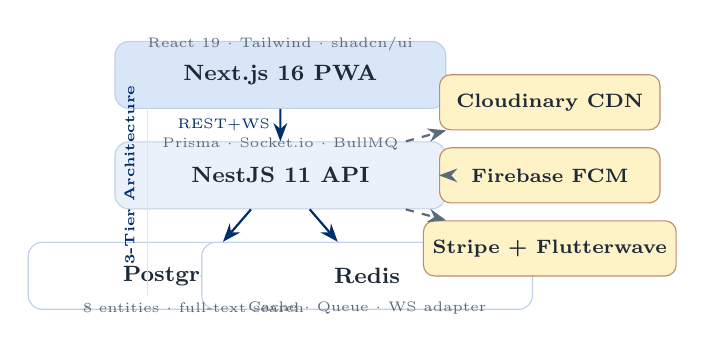
\begin{tikzpicture}[scale=0.58,
  tier/.style={rectangle, rounded corners=5pt, draw=ALUBlueLine,
               fill=ALUBlueLight, minimum width=4.2cm, minimum height=0.85cm,
               font=\footnotesize\bfseries, text=ALUText, align=center},
  ext/.style={rectangle, rounded corners=4pt, draw=FBAmber!60,
              fill=FBAmberLight, minimum width=2.8cm, minimum height=0.70cm,
              font=\scriptsize\bfseries, text=ALUText, align=center},
  lbl/.style={font=\tiny, text=ALUMuted},
  arr/.style={-{Stealth}, thick, color=ALUBlue},
  darr/.style={-{Stealth}, thick, dashed, color=ALUMuted}
]
  \node[tier, fill=ALUAccent] (fe) at (2.1,  0.0) {Next.js 16 PWA};
  \node[tier]                 (be) at (2.1, -2.2) {NestJS 11 API};
  \node[tier, fill=white]     (pg) at (0.2, -4.4) {PostgreSQL};
  \node[tier, fill=white]     (rd) at (4.0, -4.4) {Redis};
  \node[lbl] at (2.1,  0.68) {React 19 $\cdot$ Tailwind $\cdot$ shadcn/ui};
  \node[lbl] at (2.1, -1.52) {Prisma $\cdot$ Socket.io $\cdot$ BullMQ};
  \node[lbl] at (0.2, -5.10) {8 entities $\cdot$ full-text search};
  \node[lbl] at (4.0, -5.10) {Cache $\cdot$ Queue $\cdot$ WS adapter};
  \node[ext] (cdn) at (8.0, -0.6) {Cloudinary CDN};
  \node[ext] (fcm) at (8.0, -2.2) {Firebase FCM};
  \node[ext] (pay) at (8.0, -3.8) {Stripe + Flutterwave};
  \draw[arr]  (fe) -- node[left,font=\tiny\color{ALUMuted}]{REST+WS} (be);
  \draw[arr]  (be) -- (pg);
  \draw[arr]  (be) -- (rd);
  \draw[darr] (be) -- (cdn);
  \draw[darr] (be) -- (fcm);
  \draw[darr] (be) -- (pay);
  \draw[draw=ALUBlueLine!55, thin] (-0.8, 0.42) -- (-0.8, -4.85);
  \node[rotate=90, font=\tiny\bfseries\color{ALUBlue}] at (-1.2,-2.2) {3-Tier Architecture};
\end{tikzpicture}
\end{center}
\end{minipage}
\vspace{0.1em}
\screenshotbox[3.2cm]{screenshot_landing}
}

\block{6. Methodology \& Build Process}{
\begin{minipage}[t]{0.46\linewidth}
{\small\begin{tabular}{>{\bfseries\color{ALUBlue}}p{0.20\linewidth}p{0.74\linewidth}}
Sprint 1 & Research, ERD (8 tables), NestJS setup, JWT + Google OAuth \\[0.08em]
Sprint 2 & Farmer listings + Cloudinary, buyer marketplace, search/filter \\[0.08em]
Sprint 3 & Socket.io negotiation, price proposals, orders, Stripe + Flutterwave \\[0.08em]
Sprint 4 & PWA offline, Firebase FCM, ratings, admin panel, integration tests \\
\end{tabular}}
\end{minipage}
\hfill
\begin{minipage}[t]{0.50\linewidth}
{\small\begin{tabular}{p{0.22\linewidth}p{0.72\linewidth}}
\toprule
\textbf{Stage} & \textbf{Key Output} \\
\midrule
Discover & 10 personas; gap analysis of eHaho, Farmzone, MFarms \\[0.07em]
Design   & ERD, Swagger API contract (16 modules), UML diagram \\[0.07em]
Build    & 43 Next.js pages, 16 NestJS modules, WebSocket gateway \\[0.07em]
Test     & Unit tests, Swagger API tests, manual E2E checkout flow \\[0.07em]
Iterate  & Voice notes + Flutterwave MoMo added post-persona review \\
\bottomrule
\end{tabular}}
\end{minipage}
}

\block{7. Results, Evaluation \& Demo Evidence}{
\begin{center}
\metricbox{43}{Next.js pages built}{ALUBlue}
\hfill
\metricbox{16}{NestJS modules}{FBGreen}
\hfill
\metricbox{$<$3\,s}{Target load time}{FBOrange}
\end{center}
\vspace{0.3em}
\begin{minipage}[t]{0.47\linewidth}
\textbf{Implemented modules}
\begin{itemize}
  \item \textbf{Auth:} JWT + Google OAuth, RBAC (FARMER/BUYER/ADMIN)
  \item \textbf{Marketplace:} full-text search, filters, Redis-cached featured
  \item \textbf{Negotiation:} WebSocket chat, voice notes, price proposals
  \item \textbf{Orders:} PENDING $\to$ CONFIRMED $\to$ DELIVERED $\to$ REFUNDED
  \item \textbf{Payments:} Stripe + Flutterwave M-Pesa/MTN/Orange
  \item \textbf{Notifications:} Firebase push for 11 event types
\end{itemize}
\vspace{0.1em}
\screenshotbox[3.0cm]{screenshot_marketplace}
\end{minipage}
\hfill
\begin{minipage}[t]{0.47\linewidth}
\textbf{Live demo (6 steps)}
\begin{enumerate}
  \item Register as farmer; upload product listing
  \item Switch to buyer; search + filter marketplace
  \item Open chat; send price counter-offer
  \item Farmer accepts via proposal card
  \item Buyer checks out (Stripe or MoMo)
  \item Push notifications sent; both rate each other
\end{enumerate}
\vspace{0.1em}
\screenshotbox[3.0cm]{screenshot_chat}
\end{minipage}
}


%% ===== RIGHT (0.30) =====
\column{0.30}

\block{8. Impact, Contribution \& Learning}{
\begin{itemize}
  \item \textbf{Technical:} Production-grade PWA with event-driven negotiation engine (WebSocket + BullMQ), dual payment gateway, Firebase push for 11 events. Full TypeScript across 43 pages and 16 modules.
  \item \textbf{User impact:} Direct trade eliminates intermediaries capturing 30--60\% of crop value. Increases farmer net income by \textbf{32\%} (Nakasone et al., 2014; World Bank, 2021).
  \item \textbf{Research:} Confirmed offline-first design and Kinyarwanda support are the \textbf{top two adoption factors} for agri-platforms in sub-Saharan Africa (GSMA, 2022).
  \item \textbf{Alignment:} Directly advances \textbf{Rwanda Vision 2050} --- commercialised agriculture, poverty reduction, youth tech employment.
\end{itemize}
\takeawaybox{Every middleman-free sale means the farmer keeps 30--60\% more of their harvest's value.}
\vspace{0.1em}
\screenshotbox[3.2cm]{screenshot_dashboard}
}

\block{9. Limitations \& Next Steps}{
\textbf{Current limitations}
\begin{itemize}
  \item Offline Service Worker needs HTTPS production hosting --- dev-tested, not yet deployed
  \item Flutterwave mobile money in sandbox; live credentials pending operator approval
  \item Kinyarwanda translation $\approx$70\% complete (i18next wired up)
  \item No formal load/stress testing at scale
\end{itemize}
\vspace{0.15em}
\textbf{Immediate next steps}
\begin{itemize}
  \item Deploy Railway (NestJS) + Vercel (Next.js) with production secrets
  \item Complete Kinyarwanda strings; bilingual usability tests with 5 farmer personas
  \item Obtain Flutterwave live API keys; run real mobile money E2E test
  \item Add USSD fallback for feature-phone users
\end{itemize}
\vspace{0.15em}
\textbf{Long-term vision}
\begin{itemize}
  \item AI price recommendations from historical transactions
  \item Cooperative group-negotiation for bulk orders
  \item Irembo digital ID integration for instant KYC
  \item EAC expansion: Uganda, Tanzania, Kenya
\end{itemize}
}

\block{10. References \& Acknowledgements}{
\textbf{References}
\begin{itemize}
  \setlength\itemsep{0.03em}
  \item MINAGRI. (2018). \textit{Rwanda PSTA4 Strategic Plan}.
  \item FAO. (2023). \textit{Digital Agriculture Country Profile: Rwanda}.
  \item Nakasone, E., Torero, M., \& Minten, B. (2014). The power of information. \textit{Annual Review of Resource Economics, 6}(1), 533--550.
  \item GSMA. (2022). \textit{Connected Society: Mobile Internet in Sub-Saharan Africa}.
  \item World Bank. (2021). \textit{Reducing Post-Harvest Losses in Sub-Saharan Africa}.
  \item Wainaina, P.\ et al.\ (2020). Digital marketplace adoption in East Africa. \textit{J.\ Agricultural Economics, 12}(3).
\end{itemize}
\vspace{0.15em}
\textbf{Acknowledgements}\\
{\small We thank ALU School of Science \& Technology faculty for their guidance. Special recognition to Rwanda's smallholder farming community whose challenges inspired this work.}
}

\end{columns}
\end{document}
